%=====================================================================
% MONTAGEM PREDIAL - ESQUEMAS DE LIGACAO E INTERPRETACAO
%=====================================================================

\section{Esquemas de ligação e leitura de bornes}

\begin{frame}{Da prancha à ligação: sequência de leitura}
\centering
\begin{tikzpicture}[
  b/.style={draw=corPrim,fill=corDef!7,rounded corners,minimum width=1.95cm,minimum height=0.72cm,align=center,font=\scriptsize},
  a/.style={-{Stealth},thick,corPrim}]
\node[b](p)at(-5.2,0){Planta\\onde está};
\node[b](q)at(-2.6,0){Quadro de cargas\\de onde vem};
\node[b](d)at(0,0){Diagrama\\como funciona};
\node[b](b)at(2.6,0){Bornes e cabos\\como ligar};
\node[b](t)at(5.2,0){Ensaios\\como provar};
\draw[a](p)--(q)--(d)--(b)--(t);
\end{tikzpicture}
\vspace{5mm}
\begin{caixaAt}
Antes de tocar no condutor, identifique origem, proteção, tensão, polos, função de cada borne, trajeto, seção e estado de desenergização. Cor ajuda, mas etiqueta e medição controlada confirmam.
\end{caixaAt}
\end{frame}

\begin{frame}{Função dos condutores — o nome vem antes da cor}
\scriptsize
\begin{tabularx}{\textwidth}{>{\bfseries}p{2.35cm}p{2.3cm}X X}
\toprule
Função & Identificação usual & Origem/destino & Erro crítico \\
\midrule
Fase permanente & cor permitida e etiqueta F/L & proteção até comando ou carga & interromper apenas neutro \\
Neutro & azul-claro & barra N até carga que o utiliza & compartilhar entre DRs/circuitos \\
PE & verde-amarelo & barra PE até todas as massas & usar como condutor ativo \\
Retorno & cor distinta e etiqueta R & saída do comando até carga & confundir com fase permanente \\
Viajantes & par identificado V1/V2 & entre interruptores paralelos/intermediários & misturar com comum \\
Comando & código do esquema & sensor/botoeira/relé/contator & aplicar tensão errada à entrada \\
\bottomrule
\end{tabularx}
\begin{caixaAt}
Não “descobrir” função energizando fios soltos. Rastrear por documentação, identificação e ensaios previstos para instalação desenergizada.
\end{caixaAt}
\end{frame}

\begin{frame}{Ponto de luz simples — quatro representações coerentes}
\scriptsize
\begin{columns}[T,onlytextwidth]
\column{0.24\textwidth}
\centering\textbf{Funcional}\par\vspace{1mm}
\begin{circuitikz}[scale=0.58,transform shape]
\draw (0,2.8)node[left]{F} to[ospst,l=$S_1$] (2.2,2.8) to[lamp,l=$L_1$] (2.2,0) node[left]{N};
\end{circuitikz}
\column{0.24\textwidth}
\centering\textbf{Multifilar}\par\vspace{1mm}
\begin{tikzpicture}[scale=0.50]
\draw[corPrim,thick](-0.3,3)--(1,3);
\draw (1,2.7)rectangle(2.4,3.3);\node[font=\tiny]at(1.7,3){S1};
\draw[corAccent,thick](2.4,3)--(3.4,3)--(3.4,1.2);
\draw (3.4,1.0)circle(0.25);\draw(3.22,.82)--(3.58,1.18);\draw(3.22,1.18)--(3.58,.82);
\draw[corDef,thick](-0.3,0.5)--(3.4,0.5)--(3.4,.75);
\draw[corNorma,thick](-0.3,0)--(3.8,0)--(3.8,1.0);
\node[font=\tiny,anchor=east]at(-.3,3){F};\node[font=\tiny,anchor=east]at(-.3,.5){N};\node[font=\tiny,anchor=east]at(-.3,0){PE};
\end{tikzpicture}
\column{0.24\textwidth}
\centering\textbf{Caixas}\par\vspace{1mm}
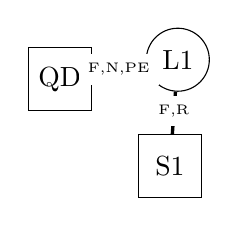
\begin{tikzpicture}[scale=0.50]
\node[draw,minimum size=.8cm](q)at(0,2.5){QD};
\node[draw,minimum size=.8cm](s)at(2.8,.3){S1};
\node[draw,circle,minimum size=.8cm](l)at(3.0,3){L1};
\draw[very thick](q)--(l);\draw[very thick](l)--(s);
\node[font=\tiny,fill=white]at(1.5,2.75){F,N,PE};
\node[font=\tiny,fill=white]at(2.9,1.7){F,R};
\end{tikzpicture}
\column{0.24\textwidth}
\centering\textbf{Bornes}\par\vspace{1mm}
\begin{tikzpicture}[scale=0.50]
\node[draw,minimum width=1.5cm,minimum height=.9cm](s)at(0,0){S1\quad L\;1};
\node[draw,circle,minimum size=.9cm](l)at(0,3){L1};
\draw[corPrim,thick](-1.5,0)--(s.west);\node[font=\tiny]at(-1.2,.3){F};
\draw[corAccent,thick](s.east)--(1.2,0)--(1.2,3)--(l.east);\node[font=\tiny]at(1.5,1.4){R};
\draw[corDef,thick](-1.5,3.35)--(l.north);\node[font=\tiny]at(-1.25,3.6){N};
\draw[corNorma,thick](-1.5,2.65)--(l.south);\node[font=\tiny]at(-1.2,2.35){PE};
\end{tikzpicture}
\end{columns}
\vspace{2mm}
\begin{caixaObs}
As quatro vistas descrevem o mesmo circuito. Se uma delas exigir condutor ou borne que não aparece nas demais, há incompatibilidade a resolver.
\end{caixaObs}
\end{frame}

\begin{frame}{Ponto simples — condutores por trecho}
\centering
\begin{tikzpicture}[scale=0.82,every node/.style={font=\scriptsize}]
\node[draw=corPrim,fill=corDef!7,minimum width=1.4cm,minimum height=.8cm](q)at(-4.8,1.8){QD / C1};
\node[draw=corPrim,circle,minimum size=1.0cm,align=center](cx)at(0,1.8){caixa\\de teto};
\node[draw=corNorma,fill=corNorma!7,minimum width=1.4cm,minimum height=.8cm](s)at(4.8,-1.0){S1};
\node[draw=corAccent,circle,minimum size=.8cm](l)at(4.8,3.6){L1};
\draw[very thick](q)--(cx);\draw[very thick](cx)--(l);\draw[very thick](cx)--(s);
\node[fill=white,align=center]at(-2.4,2.15){F + N + PE\\3 x 1,5 mm$^2$};
\node[fill=white,align=center]at(2.4,3.05){R + N + PE\\3 x 1,5 mm$^2$};
\node[fill=white,align=center]at(2.25,0.15){F + R\\2 x 1,5 mm$^2$};
\end{tikzpicture}
\vspace{1mm}
\begin{caixaAt}
O PE acompanha o circuito até a luminária e demais massas, mesmo quando não entra no mecanismo do interruptor. O trecho ao interruptor muda se houver sensor, automação ou dispositivo que também necessite de neutro.
\end{caixaAt}
\end{frame}

\begin{frame}{Interruptor duplo — dois retornos, um comum identificado}
\small
\begin{columns}[T,onlytextwidth]
\column{0.51\textwidth}
\begin{tikzpicture}[scale=0.78]
\node[draw=corNorma,fill=corNorma!7,minimum width=2.3cm,minimum height=1.4cm](s)at(0,0){S1a\qquad S1b};
\node[draw,circle,minimum size=.9cm](l1)at(4.2,1.7){L1};
\node[draw,circle,minimum size=.9cm](l2)at(4.2,-1.7){L2};
\draw[corPrim,thick](-2.4,0)--(s.west);\node[font=\scriptsize]at(-2.0,.35){F};
\draw[corAccent,thick](s.north east)--(2.1,.7)--(2.1,1.7)--(l1.west);\node[font=\tiny]at(2.35,1.15){R1};
\draw[corFix,thick](s.south east)--(2.1,-.7)--(2.1,-1.7)--(l2.west);\node[font=\tiny]at(2.35,-1.15){R2};
\draw[corDef,thick](-2.4,2.4)--(4.2,2.4)--(l1.north);
\draw[corDef,thick](4.2,2.4)--(4.2,-1.25);
\draw[corNorma,thick](-2.4,-2.4)--(4.65,-2.4)--(4.65,-1.7);
\end{tikzpicture}
\column{0.47\textwidth}
\begin{enumerate}
\item identificar o borne comum do conjunto;
\item alimentar a ponte somente se o fabricante permitir;
\item ligar R1 e R2 às cargas corretas;
\item manter N e PE nas caixas das luminárias;
\item etiquetar ambos os retornos;
\item testar cada tecla e a correspondência com a planta.
\end{enumerate}
\end{columns}
\begin{caixaAt}
Não unir saídas para “somar potência”. Cada tecla e seu borne têm corrente e tipo de carga admissíveis definidos pelo fabricante.
\end{caixaAt}
\end{frame}

\begin{frame}{Comando paralelo — uma luz em dois locais}
\centering
\begin{tikzpicture}[scale=0.90,every node/.style={font=\scriptsize}]
\node[draw=corNorma,fill=corNorma!7,minimum width=1.7cm,minimum height=2.2cm,align=center](s1)at(-3.6,0){S1\\paralelo};
\node[draw=corNorma,fill=corNorma!7,minimum width=1.7cm,minimum height=2.2cm,align=center](s2)at(1.0,0){S2\\paralelo};
\node[draw,circle,minimum size=1.0cm](l)at(4.8,0){L1};
\fill (-4.45,0)circle(2.2pt);\node[font=\tiny]at(-4.15,.25){C};
\fill (-2.75,.65)circle(2.2pt);\fill (-2.75,-.65)circle(2.2pt);
\fill (.15,.65)circle(2.2pt);\fill(.15,-.65)circle(2.2pt);\fill(1.85,0)circle(2.2pt);\node[font=\tiny]at(1.55,.25){C};
\draw[corPrim,thick](-5.8,0)--(-4.45,0);\node[font=\scriptsize]at(-5.45,.35){F};
\draw[corAccent,thick](-2.75,.65)--(.15,.65);\node[font=\tiny]at(-1.3,.9){V1};
\draw[corFix,thick](-2.75,-.65)--(.15,-.65);\node[font=\tiny]at(-1.3,-.9){V2};
\draw[corPrim,thick](-4.45,0)--(-2.75,.65);
\draw[corPrim,thick](.15,.65)--(1.85,0);
\draw[corAccent,thick](1.85,0)--(l.west);\node[font=\tiny]at(3.05,.3){R};
\draw[corDef,thick](-5.8,2.1)--(4.8,2.1)--(l.north);\node[font=\tiny]at(-5.45,2.35){N};
\draw[corNorma,thick](-5.8,-2.1)--(4.8,-2.1)--(l.south);\node[font=\tiny]at(-5.45,-2.35){PE};
\end{tikzpicture}
\begin{caixaProjeto}[title=Leitura dos bornes]
Fase entra no comum de S1; V1 e V2 ligam os pares viajantes; o comum de S2 fornece o retorno à luminária. O borne comum deve ser identificado no mecanismo, não inferido pela posição.
\end{caixaProjeto}
\end{frame}

\begin{frame}{Comando intermediário — uma luz em três ou mais locais}
\centering
\begin{tikzpicture}[scale=0.80,every node/.style={font=\scriptsize}]
\node[draw=corNorma,fill=corNorma!7,minimum width=1.6cm,minimum height=2.0cm,align=center](s1)at(-5.0,0){S1\\paralelo};
\node[draw=corDef,fill=corDef!7,minimum width=2.0cm,minimum height=2.2cm,align=center](si)at(0,0){S2\\intermediário};
\node[draw=corNorma,fill=corNorma!7,minimum width=1.6cm,minimum height=2.0cm,align=center](s3)at(5.0,0){S3\\paralelo};
\draw[corPrim,thick](-7.0,0)--(s1.west);\node[font=\tiny]at(-6.6,.25){F no comum};
\draw[corAccent,thick](s1.north east)--(si.north west);
\draw[corFix,thick](s1.south east)--(si.south west);
\draw[corAccent,thick](si.north west)--(si.south east);
\draw[corFix,thick](si.south west)--(si.north east);
\draw[corAccent,thick](si.north east)--(s3.north west);
\draw[corFix,thick](si.south east)--(s3.south west);
\draw[corAccent,thick](s3.east)--(7.0,0);\node[font=\tiny]at(6.45,.3){R no comum};
\node[font=\tiny,corPrim]at(-2.5,1.25){par viajante};\node[font=\tiny,corPrim]at(2.5,1.25){par viajante};
\end{tikzpicture}
\vspace{2mm}
\begin{caixaObs}
O intermediário apenas comuta/cruza os dois viajantes e fica entre dois paralelos. Para quatro pontos de comando, inserir outro intermediário em série no par viajante.
\end{caixaObs}
\begin{caixaAt}
Não usar mecanismo simples no lugar do intermediário. Conferir o diagrama impresso e identificar os dois pares de bornes antes da ligação.
\end{caixaAt}
\end{frame}

\begin{frame}{Botoeiras e relé de impulso — muitos pontos de comando}
\centering
\begin{tikzpicture}[
  b/.style={draw=corPrim,fill=corDef!7,rounded corners,minimum width=1.8cm,minimum height=.65cm,align=center,font=\scriptsize}]
\node[b](dj)at(-5.2,2.0){DJ C1};
\node[b](ct)at(-2.4,2.0){Contato do relé};
\node[b](l)at(.3,2.0){Luminárias};
\draw[-{Stealth},thick,corPrim](dj)--(ct)--(l);
\node[b,draw=corNorma,fill=corNorma!7](bob)at(-2.4,-1.2){Bobina A1--A2};
\node[b](b1)at(1.0,-.5){B1};\node[b](b2)at(3.1,-1.2){B2};\node[b](bn)at(5.2,-.5){Bn};
\draw[corPrim,thick](-5.2,-1.2)--(bob);
\draw[corAccent,thick](bob)--(b1);\draw[corAccent,thick](bob)--(b2);\draw[corAccent,thick](bob)--(bn);
\node[font=\tiny,align=center]at(2.95,-2.0){botoeiras momentâneas em paralelo};
\draw[dashed,corNorma,-{Stealth}](bob)--(ct);
\end{tikzpicture}
\vspace{3mm}
\begin{caixaAt}
Tensão da bobina, contato admissível e esquema A1/A2 variam. Botoeira não alimenta diretamente a luminária: envia um pulso ao relé, que comuta a carga.
\end{caixaAt}
\end{frame}

\begin{frame}{Sensor de presença — ler L, N e saída comutada}
\small
\begin{columns}[T,onlytextwidth]
\column{0.52\textwidth}
\begin{tikzpicture}[scale=0.86]
\node[draw=corNorma,fill=corNorma!7,minimum width=2.4cm,minimum height=1.5cm,align=center](sen)at(0,0){SENSOR\\L\quad N\quad L$'$};
\node[draw,circle,minimum size=1.0cm](l)at(4.4,0){L1};
\draw[corPrim,thick](-3,0.45)--(sen.west |- 0,0.45);\node[font=\tiny]at(-2.6,.75){F/L};
\draw[corDef,thick](-3,-.45)--(sen.west |- 0,-.45);\node[font=\tiny]at(-2.6,-.75){N};
\draw[corAccent,thick](sen.east)--(l.west);\node[font=\tiny]at(2.8,.3){L$'$};
\draw[corDef,thick](-3,-1.6)--(4.4,-1.6)--(l.south);
\draw[corNorma,thick](-3,-2.1)--(4.8,-2.1)--(4.8,0);
\end{tikzpicture}
\column{0.46\textwidth}
\begin{itemize}
\item alguns modelos exigem neutro; outros são de dois fios;
\item respeitar potência mínima/máxima e tipo de carga LED;
\item selecionar tempo, nível de luz e sensibilidade;
\item evitar campo bloqueado, calor e fluxo direto de ar;
\item usar contator/relé quando a carga ou corrente de partida exigir.
\end{itemize}
\end{columns}
\end{frame}

\begin{frame}{Fotocélula — comando externo com alimentação permanente}
\centering
\begin{tikzpicture}[scale=0.88,every node/.style={font=\scriptsize}]
\node[draw=corPrim,fill=corDef!7,minimum width=1.8cm,minimum height=.7cm](dj)at(-5,0){DJ};
\node[draw=corNorma,fill=corNorma!7,minimum width=2.4cm,minimum height=1.4cm,align=center](fc)at(-1.5,0){FOTOCÉLULA\\L\quad N\quad L$'$};
\node[draw=corDef,fill=corDef!7,minimum width=1.8cm,minimum height=.7cm,align=center](k)at(2,0){Relé/contator\\se necessário};
\node[draw,circle,minimum size=.9cm](l)at(5,0){fachada};
\draw[-{Stealth},thick,corPrim](dj)--(fc)--(k)--(l);
\draw[corDef,thick](-5,-1.5)--(-1.5,-1.5)--(-1.5,-.72);
\draw[corDef,thick](-1.5,-1.5)--(5,-1.5)--(l.south);
\node[font=\tiny,corDef]at(-4.6,-1.75){N};
\draw[corNorma,thick](-5,-2)--(5.4,-2)--(5.4,0);
\end{tikzpicture}
\begin{caixaObs}
Instalar o sensor onde a própria luminária não provoque ciclos de liga/desliga. Programação por relógio/automação pode limitar horário, mas a função de cada dispositivo deve aparecer no diagrama.
\end{caixaObs}
\end{frame}

\begin{frame}{Dimmer e driver LED — compatibilidade é de sistema}
\scriptsize
\begin{tabularx}{\textwidth}{>{\bfseries}p{2.6cm}X X}
\toprule
Interface & Condutores típicos & Conferir \\
\midrule
Corte de fase & fase, saída dimerizada e às vezes neutro & tipo de borda, potência mínima, ruído e lista de drivers \\
0--10 V & força + par de controle polarizado & fonte/sumidouro, segregação e falha do controle \\
DALI & força permanente + barramento de dois fios & endereços, grupos, fonte do barramento e comissionamento \\
PWM/baixa tensão & alimentação + sinal do fabricante & distância, seção, frequência e compatibilidade \\
Relé liga/desliga & força comutada & corrente de partida e número de drivers \\
\bottomrule
\end{tabularx}
\begin{caixaAt}
“LED dimerizável” não garante compatibilidade. Validar luminária + driver + comando + faixa de dimerização e realizar mockup quando o resultado visual for crítico.
\end{caixaAt}
\end{frame}

\begin{frame}{Tomada 2P+T — vista frontal não é vista dos bornes}
\small
\begin{columns}[T,onlytextwidth]
\column{0.48\textwidth}
\centering\textbf{Vista do usuário}\par
\begin{tikzpicture}[scale=0.86]
\draw[very thick,rounded corners](-2,-2)rectangle(2,2);
\draw[corPrim,fill=corPrim!10](-.7,.5)circle(.18);\node[font=\tiny]at(-.7,.95){polo};
\draw[corDef,fill=corDef!10](.7,.5)circle(.18);\node[font=\tiny]at(.7,.95){polo};
\draw[corNorma,fill=corNorma!10](0,-.75)circle(.20);\node[font=\tiny]at(0,-1.2){terra};
\end{tikzpicture}
\column{0.50\textwidth}
\centering\textbf{Vista de ligação}\par
\begin{tikzpicture}[scale=0.86]
\draw[very thick,rounded corners](-2,-2)rectangle(2,2);
\node[draw,circle,minimum size=.65cm]at(-.9,.6){L};
\node[draw,circle,minimum size=.65cm]at(.9,.6){N};
\node[draw,circle,minimum size=.65cm]at(0,-.8){PE};
\draw[corPrim,thick](-2.8,.6)--(-1.25,.6);
\draw[corDef,thick](2.8,.6)--(1.25,.6);
\draw[corNorma,thick](0,-2.8)--(0,-1.15);
\end{tikzpicture}
\end{columns}
\begin{caixaAt}
Orientação de L/N pode depender do padrão adotado e da marcação do mecanismo. Conferir gravação e ficha do fabricante; nunca deduzir os bornes olhando apenas a frente da tomada.
\end{caixaAt}
\end{frame}

\begin{frame}{“220 V” pode ser fase--neutro ou fase--fase}
\small
\begin{columns}[T,onlytextwidth]
\column{0.49\textwidth}
\begin{caixaProjeto}[title=220 V fase--neutro]
\begin{tikzpicture}[scale=.72]
\node[draw,minimum width=2cm,align=center](q)at(0,1){DJ 1P/2P\\conforme projeto};
\node[draw,minimum width=2cm](c)at(4,1){carga 220 V};
\draw[corPrim,thick](q)--(c);\draw[corDef,thick](0,0)--(4,0)--(c.south);
\node[font=\tiny]at(2,1.25){F};\node[font=\tiny]at(2,.25){N};
\end{tikzpicture}
Neutro participa do circuito e deve ser identificado/protegido/seccionado conforme o esquema aplicável.
\end{caixaProjeto}
\column{0.49\textwidth}
\begin{caixaProjeto}[title=220 V fase--fase]
\begin{tikzpicture}[scale=.72]
\node[draw,minimum width=2cm](q)at(0,1){DJ 2P};
\node[draw,minimum width=2cm](c)at(4,1){carga 220 V};
\draw[corPrim,thick](q.north east)--(c.north west);\draw[corFix,thick](q.south east)--(c.south west);
\node[font=\tiny]at(2,1.55){F1};\node[font=\tiny]at(2,.45){F2};
\end{tikzpicture}
Não existe neutro na alimentação da carga; ambos os condutores ativos devem ser tratados como fase.
\end{caixaProjeto}
\end{columns}
\begin{caixaAt}
Confirmar tensão entre condutores, sistema do edifício e diagrama. Nunca ligar por memória de cores ou por “aqui sempre foi assim”.
\end{caixaAt}
\end{frame}

\begin{frame}{Chuveiro/aquecedor — circuito dedicado e conexão correta}
\centering
\begin{tikzpicture}[
  b/.style={draw=corPrim,fill=corDef!7,rounded corners,minimum width=2.2cm,minimum height=.75cm,align=center,font=\scriptsize}]
\node[b](q)at(-4.5,0){QD\\DJ 2P + DR};
\node[b](cx)at(-1.5,0){Caixa de conexão\\fora do jato};
\node[b](c)at(1.5,0){Conector\\para carga e seção};
\node[b](a)at(4.5,0){Aquecedor\\bornes ativos + PE};
\draw[-{Stealth},thick,corPrim](q)--(cx)--(c)--(a);
\draw[corNorma,thick](q.south)--(-4.5,-1.3)--(4.5,-1.3)--(a.south);
\node[font=\tiny,corNorma]at(0,-1.55){PE contínuo até o borne de proteção};
\end{tikzpicture}
\vspace{3mm}
\begin{itemize}
\item conferir placa, tensão, potência, corrente, seção e proteção;
\item não usar tomada/plugue comum se o fabricante exigir conexão fixa;
\item não estanhar pontas; usar terminal/conector aceito;
\item preservar volume de segurança e grau de proteção;
\item realizar ensaios antes da energização funcional.
\end{itemize}
\end{frame}

\begin{frame}{Ar-condicionado split — força e interligação são documentos distintos}
\small
\begin{columns}[T,onlytextwidth]
\column{0.54\textwidth}
\begin{tikzpicture}[scale=.70,every node/.style={font=\scriptsize}]
\node[draw=corPrim,fill=corDef!7,minimum width=1.5cm,minimum height=.7cm](qd)at(-4.5,1.4){QD};
\node[draw=corNorma,fill=corNorma!7,minimum width=1.6cm,minimum height=.7cm](sc)at(-2.0,1.4){seccionador};
\node[draw=corPrim,minimum width=2cm,minimum height=1.1cm,align=center](ue)at(.6,1.4){unidade\\externa};
\node[draw=corDef,minimum width=2cm,minimum height=1.1cm,align=center](ui)at(4.2,1.4){unidade\\interna};
\draw[-{Stealth},thick,corPrim](qd)--(sc)--(ue);
\draw[corNorma,thick](qd.south)--(-4.5,0)--(.6,0)--(ue.south);
\draw[corFix,thick,<->](ue)--(ui);\node[font=\tiny,align=center]at(2.4,1.85){interligação\\do fabricante};
\end{tikzpicture}
\column{0.44\textwidth}
\begin{itemize}
\item origem da alimentação pode ser unidade interna ou externa;
\item cabo entre unidades pode misturar força e comunicação conforme projeto do produto;
\item número e código dos bornes devem coincidir nas duas extremidades;
\item prever seccionamento e acesso de manutenção;
\item proteger e vedar a passagem sem criar dreno para água.
\end{itemize}
\end{columns}
\end{frame}

\begin{frame}{Bomba com boia — separar potência e comando}
\scriptsize
\begin{columns}[T,onlytextwidth]
\column{0.49\textwidth}
\centering\textbf{Potência}\par\vspace{1mm}
\begin{tikzpicture}[scale=.68]
\node[draw,minimum width=2cm](dj)at(0,3){DJ motor};
\node[draw,minimum width=2cm](k)at(0,1.8){K1 contatores};
\node[draw,minimum width=2cm](rt)at(0,.6){relé térmico};
\node[draw,circle,minimum size=1cm](m)at(0,-.8){M};
\draw[-{Stealth},thick,corPrim](dj)--(k)--(rt)--(m);
\end{tikzpicture}
\column{0.49\textwidth}
\centering\textbf{Comando automático/manual}\par\vspace{1mm}
\begin{tikzpicture}[scale=.68]
\node[draw,minimum width=1.8cm](s0)at(-3,2.4){S0 para};
\node[draw,minimum width=1.8cm](sel)at(0,2.4){MAN--0--AUTO};
\node[draw,minimum width=1.8cm](b)at(3,3.2){boia};
\node[draw,minimum width=1.8cm](s1)at(3,1.6){S1 liga};
\node[draw,minimum width=1.8cm](coil)at(0,.2){bobina K1};
\draw[-{Stealth},thick,corPrim](s0)--(sel);\draw[-{Stealth},thick,corPrim](sel)--(b);\draw[-{Stealth},thick,corPrim](sel)--(s1);\draw[-{Stealth},thick,corPrim](b)--(coil);\draw[-{Stealth},thick,corPrim](s1)--(coil);
\end{tikzpicture}
\end{columns}
\begin{caixaAt}
Boia deve comandar a bobina dentro de sua capacidade, não necessariamente a corrente do motor. Incluir proteção contra falta de água, sobrecarga e condição de falha conforme o processo.
\end{caixaAt}
\end{frame}

\begin{frame}{Campainha, interfone e dados — manter separação funcional}
\centering
\begin{tikzpicture}[
  b/.style={draw=corPrim,fill=corDef!7,rounded corners,minimum width=2.2cm,minimum height=.72cm,align=center,font=\scriptsize}]
\node[b](rede)at(-4.5,1.5){230/220 V\\circuito protegido};
\node[b](fonte)at(-1.5,1.5){Fonte SELV/PELV\\quando aplicável};
\node[b](bot)at(1.5,2.4){botoeira / painel};
\node[b](int)at(4.5,1.5){interfone / campainha};
\node[b](fech)at(1.5,.2){fechadura elétrica};
\draw[-{Stealth},thick,corPrim](rede)--(fonte);
\draw[-{Stealth},thick,corDef](fonte)--(bot)--(int);
\draw[-{Stealth},thick,corDef](bot)--(fech);
\draw[dashed,corAt,very thick] (0,-1) -- (0,3.4);
\node[font=\tiny,corAt,rotate=90]at(.25,-.1){barreira / segregação};
\end{tikzpicture}
\begin{caixaObs}
Seguir o esquema do fabricante para polaridade, topologia e distância. Não compartilhar eletroduto/caixa com força sem que a solução completa atenda à isolação e segregação exigidas.
\end{caixaObs}
\end{frame}

\begin{frame}{Bloco autônomo de emergência — alimentação não comandada}
\centering
\begin{tikzpicture}[scale=.88,every node/.style={font=\scriptsize}]
\node[draw=corPrim,fill=corDef!7,minimum width=2cm,minimum height=.75cm](dj)at(-4,1.2){circuito previsto};
\node[draw=corAt,fill=corAt!8,minimum width=2.6cm,minimum height=1.3cm,align=center](bl)at(0,1.2){bloco autônomo\\rede + bateria};
\node[draw=corNorma,fill=corNorma!7,minimum width=2cm,minimum height=.75cm](lamp)at(4,1.2){LED emergência};
\draw[-{Stealth},thick,corPrim](dj)--(bl);\draw[-{Stealth},thick,corAt](bl)--(lamp);
\node[draw=corNorma,minimum width=2cm,minimum height=.65cm](test)at(0,-1.2){teste / supervisão};
\draw[dashed,-{Stealth},corNorma](test)--(bl);
\draw[corAt,very thick](-2.1,.45)--(-1.5,1.05);\draw[corAt,very thick](-2.1,1.05)--(-1.5,.45);
\node[font=\tiny,corAt]at(-2.55,.25){sem interruptor local};
\end{tikzpicture}
\begin{caixaAt}
Alimentação, proteção, supervisão, autonomia, posição e ensaios pertencem ao projeto de emergência. Não aproveitar o retorno da iluminação normal para alimentar o bloco.
\end{caixaAt}
\end{frame}

\begin{frame}{Numeração de fios e bornes — tornar o diagrama montável}
\small
\begin{columns}[T,onlytextwidth]
\column{0.55\textwidth}
\begin{tikzpicture}[scale=.78,every node/.style={font=\scriptsize}]
\node[draw,minimum width=2cm](x1)at(-3,2){X1:01};
\node[draw,minimum width=2cm](s)at(0,2){S1:L};
\node[draw,minimum width=2cm](s2)at(0,0){S1:1};
\node[draw,minimum width=2cm](x2)at(3,0){X2:07};
\draw[corPrim,thick,-{Stealth}](x1)--(s)node[midway,above]{101};
\draw[corAccent,thick,-{Stealth}](s2)--(x2)node[midway,above]{102};
\draw[dashed](s)--(s2);\node[font=\tiny]at(.55,1){contato};
\end{tikzpicture}
\column{0.43\textwidth}
\begin{itemize}
\item X1/X2: régua ou caixa de passagem;
\item 01/07: borne físico;
\item S1:L e S1:1: bornes do dispositivo;
\item 101/102: identificação do condutor;
\item folha/zona: referência cruzada do desenho;
\item cabo: origem, destino e formação na lista.
\end{itemize}
\end{columns}
\begin{caixaObs}
O mesmo código deve aparecer no diagrama, anilha/etiqueta, lista de cabos e relatório de continuidade.
\end{caixaObs}
\end{frame}

\begin{frame}{Como interpretar um esquema desconhecido}
\scriptsize
\begin{enumerate}
\item localizar título, revisão, tensão e condição de repouso;
\item marcar fonte, proteção e barramentos de referência;
\item separar potência, comando, sinal e proteção;
\item seguir um caminho de cada vez, da origem ao retorno;
\item identificar contatos pelo dispositivo que os aciona;
\item anotar bornes, fios, cabos e referências cruzadas;
\item converter a lógica em lista física de conexões;
\item comparar com placa/ficha do equipamento;
\item executar verificação ponto a ponto ainda desenergizada;
\item liberar ensaios funcionais somente pelo procedimento definido.
\end{enumerate}
\begin{caixaProjeto}[title=Pergunta obrigatória]
Se este fio for removido, qual função deixa de existir? Se a resposta não estiver clara, a ligação ainda não foi compreendida.
\end{caixaProjeto}
\end{frame}

\begin{frame}{Falhas típicas — diagnóstico pelo esquema}
\scriptsize
\begin{tabularx}{\textwidth}{>{\bfseries}p{2.9cm}X X}
\toprule
Sintoma & Hipóteses a verificar & Evidência esperada \\
\midrule
Luz não acende & proteção, fase, retorno, neutro, carga & continuidade/tensão no ponto previsto pelo procedimento \\
Paralelos “invertidos” & comum ligado a viajante & bornes C/V1/V2 não coincidem com diagrama \\
LED pisca apagado & fuga no comando, sensor/dimmer incompatível, indução & comportamento muda com dispositivo/carga de teste apropriada \\
DR desarma & N compartilhado, fuga PE, ligação N-PE a jusante & isolação e rastreio por circuito \\
Sensor não desliga & campo, tempo, ligação L/L$'$, carga mínima & parâmetros e bornes comparados à ficha \\
Motor não parte & comando aberto, térmico, bobina ou potência & cadeia de permissivos e estado de K1 \\
\bottomrule
\end{tabularx}
\begin{caixaAt}
Diagnóstico energizado exige análise de risco, instrumento adequado, procedimento e profissional autorizado. Priorizar inspeção e testes desenergizados sempre que possível.
\end{caixaAt}
\end{frame}

\begin{frame}{Prática de leitura e ligação — critério de aprovação}
\small
Para um circuito sorteado — simples, duplo, paralelo, intermediário, sensor ou relé — o aluno deve:
\begin{enumerate}
\item explicar a função sem tocar nos componentes;
\item desenhar funcional, multifilar e ligação física;
\item produzir lista de bornes e condutores por trecho;
\item selecionar seção, proteção e componentes a partir do projeto;
\item montar em bancada desenergizada e identificada;
\item verificar continuidade, ausência de curto e PE;
\item energizar somente após liberação do responsável;
\item demonstrar a função e localizar uma falha inserida;
\item atualizar o desenho conforme montado.
\end{enumerate}
\begin{caixaAt}
Acender a lâmpada não basta. Aprovação exige ligação correta, proteção preservada, documentação coerente e ensaios registrados.
\end{caixaAt}
\end{frame}
